\chapter{Zadanie 2.}
Odpowiedzi skokowe zosta�y wyznaczone poprzez zmian� sterowania z punktu pracy do warto�ci:
\begin{itemize}
\item {\color{blue}$ u = 2.4 $}
\item {\color{red}$ u = 2.8 $}
\item {\color{yellow}$ u = 1.6 $}
\item {\color{green}$ u = 1.2 $}
\end{itemize}

\begin{figure}[b]
\centering
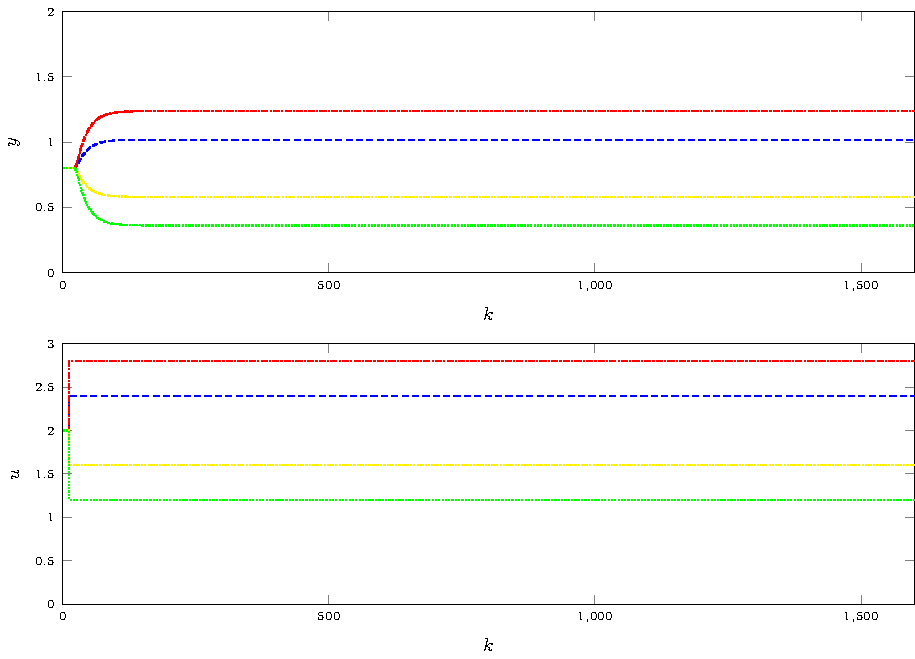
\includegraphics[scale=1]{rysunki/zapisz_pdf/proj1/reakcje.pdf}
\caption {Odpowiedzi skokowe dla r�nych warto�ci skoku}
\end{figure}

Charakterystyk� statyczn� procesu wida� na wykresie ~\ref{fig:char_stat}

\begin{figure}[b]
\centering
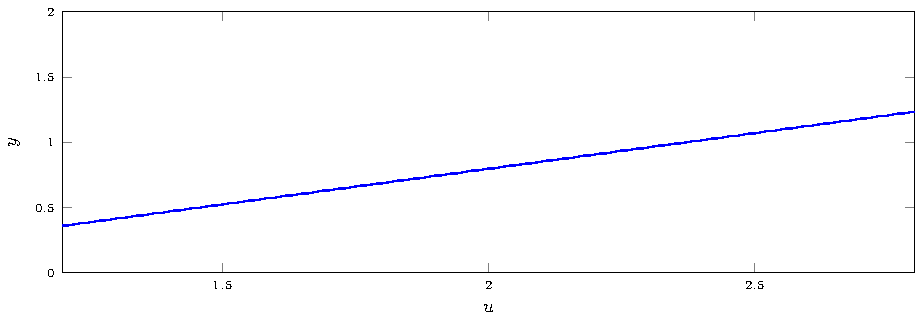
\includegraphics[scale=1]{rysunki/zapisz_pdf/proj1/charakterystyka_statyczna.pdf}
\caption {Charakterystyka statyczna}
\label{fig:char_stat}
\end{figure}
W�a�ciwo�ci statyczne i dynamiczne s� w przybli�eniu liniowe, st�d wzmocnienie statyczne zosta�o policzone za pomoc� wzoru:
$$ K = \frac{\Delta y}{\Delta u} = 0,5484 $$